\documentclass[12pt]{article}

\usepackage{fullpage}
\usepackage{multicol, multirow}
\usepackage{tabularx}
\usepackage{standalone}
\usepackage{listings}
\usepackage{ulem}
\usepackage{amsmath}
\usepackage{pdfpages}
\usepackage[utf8]{inputenc}
\usepackage[russian]{babel}

\newcommand{\StudentName}{Ильвохин Дмитрий}
\newcommand{\Group}{1O-106М}
\newcommand{\CourseName}{Программирование игр}
\newcommand{\LabNum}{4}
\newcommand{\Subject}{Космическое приключение}
\newcommand{\PrepName}{Аносова Н.\,П.}

\begin{document}

%\documentclass[a4paper, 12pt]{report}
\usepackage[english, russian]{babel}
\usepackage[utf8]{inputenc}
\usepackage{amssymb, amsfonts, amsmath, mathtext, cite, enumerate, float}
\usepackage{geometry}
\usepackage{chngpage}

\begin{document}

\begin{titlepage}

\newpage

\begin{center}
Московский Авиационный Институт \\*
(национальный исследовательский университет) \\*
Факультет прикладной математики и физики \\*
\hrulefill
\end{center}

\begin{center}
Кафедра вычислительной математики и программирования
\end{center}

\vspace{6em}

\begin{center}
\Large \CourseName \\
	Курсоваой проект \\
  <<\Subject>>
\end{center}

\vspace{2em}
\vspace{6em}

\begin{flushright}
	\StudentName, \\
	группа: \Group \\
\vspace{1em}
преподаватель:\\
   \PrepName \\
\end{flushright}

\vspace{\fill}

\begin{center}
Москва, 2015
\end{center}

\end{titlepage}

\end{document}
 % title page

\lstset
{
        language=Python,
        basicstyle=\footnotesize,% basic font setting
        extendedchars=\true
}

\begin{flushright}
\Large{
	\CourseName \\
	Лабораторная работа №\,\LabNum \\
	<<\Subject>> \\
  \StudentName, \Group \\
}
\end{flushright}

\subsection*{Задание}
Необходимо реализовать 3D игру. Действие происходит в космосе, камера смотрит
на космический корабль сзади, вокруг корабля большое количество астероидов.
Цели игрока --- управляя космическим кораблем избежать столкновения с астероидами.

\subsection*{Практическая часть}
Для выполнения лабораторной работы решил опять использовать
игровой движок Padna3D, чтобы познакомиться с ним получше.

Модель космического корабля взял из галереи готовых моделей, которую
можно скачать на официальном сайте движка.~\cite{panda}

В качестве астероидов используются модели додекаэдра~\cite{dodecahedron},
икосаэдра~\cite{icosahedron}, октаэдра~\cite{octahedron},
взятые из той же коллекции моделей, с <<каменной>> текстурой, которая делает
их хоть немного похожими на астероиды.

Для придания эффекта движения, шар с текстурой звездного неба вращается и двигаются
астероиды вокруг корабля, сам же космический корабли на самом деле не движется вперед,
только в стороны.

В самом начале создания сцены случайным образом генерируется некоторое количество астероидов,
которые движутся на встречу кораблю. Как только астероиды оказываются за камерой по оси Y ---
им генерируется новая координата в дали (тумане) и они снова помещаются перед камерой.

Для упрощения обработки коллизий все сложные (и не очень тела) обернуты в сферы подходящего
радиуса для которых и считаются коллизии. Их можно увидеть выставив в коде флаг DEBUG.

\begin{figure}[!htb]
  \centering
    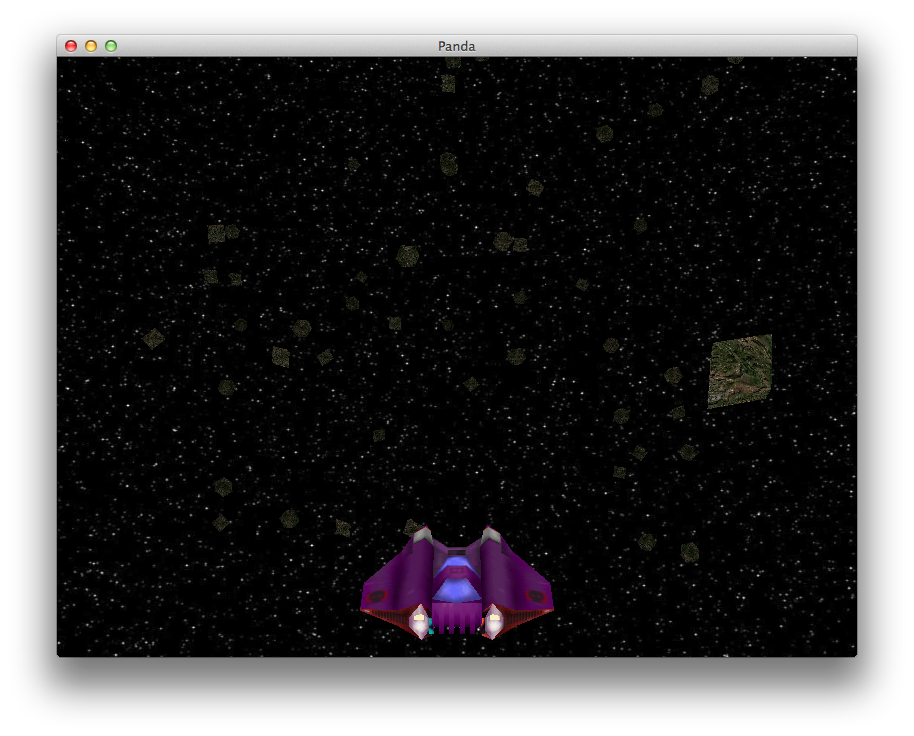
\includegraphics[scale=0.5]{pics/game.png}
   \caption{Скриншот}
    \label{fig:game}
\end{figure}

\subsection*{Выводы}

\begin{thebibliography}{}
\bibitem{panda_wiki} https://ru.wikipedia.org/wiki/Panda3D
\bibitem{panda} https://www.panda3d.org/
\bibitem{dodecahedron} https://en.wikipedia.org/wiki/Dodecahedron
\bibitem{icosahedron} https://en.wikipedia.org/wiki/Icosahedron
\bibitem{octahedron} https://en.wikipedia.org/wiki/Octahedron
\end{thebibliography}

\end{document}


